\documentclass{beamer}
\usepackage{graphicx}
\usepackage{xcolor}
\usepackage{tikz}

\usepackage{colortbl}     % 支持 \rowcolor
\usepackage[table]{xcolor}  % 增强颜色支持，特别是灰色背景
\usepackage{array}        % 增强表格功能（对齐方式等）
\usepackage{booktabs



% 自定义颜色
\definecolor{purpleblue}{RGB}{80, 80, 180}
\definecolor{lightgray}{RGB}{230, 230, 230}
\definecolor{novelPurple}{RGB}{98, 54, 255} 
\definecolor{darkgray}{RGB}{50, 50, 50}

% 主题设置
\usetheme{Madrid}  
\usecolortheme{dolphin} 

% 设置字体（移除 fontspec，确保 pdfLaTeX 兼容）
\setbeamerfont{title}{size=\Large,series=\bfseries}
\setbeamerfont{frametitle}{size=\LARGE,series=\bfseries}
\setbeamercolor{frametitle}{fg=white, bg=novelPurple}
\setbeamercolor{title}{fg=white, bg=purpleblue}
% 封面信息
\title[Enhanced Math II Unit 8]{\textbf{ Enhanced Math II\\ Unit 8}}
\author{\textbf{Jack Zeng}}
\institute{\textcolor{white}{\textbf{Novel Prep}}}
\date{\today} 

\begin{document}

% --- Title Slide ---
\begin{frame}
    \titlepage
    \vfill
    \begin{flushright}
        \textcolor{purpleblue}{\Huge \textbf{Novel Prep}}
    \end{flushright}
\end{frame}



\begin{frame}
    \begin{tikzpicture}[remember picture, overlay]
        \shade[top color=softPurple, bottom color=softGray] 
            (current page.north west) rectangle (current page.south east);
        \fill[white, opacity=0.3] (current page.center) circle (4cm);
        
        \node[align=center] at (current page.center) {
            {\Huge\bfseries\textcolor{purpleblue}{Novel Prep}} \\[0.5cm]
            {\Large\itshape\textcolor{lightText}{Excellence in SAT Prep}}
        };
        \foreach \x in {1,2,3,4,5} {
            \fill[purpleblue, opacity=0.2] (rand*10-5, rand*7-3.5) circle (0.1+\x*0.05);
        }
        ;
    \end{tikzpicture}
\end{frame}

\begin{frame}{Overview}
    \tableofcontents
\end{frame}


\begin{frame}
\section{Line}
    \begin{tikzpicture}[remember picture, overlay]
        \shade[top color=softPurple, bottom color=softGray] 
            (current page.north west) rectangle (current page.south east);
        \fill[white, opacity=0.3] (current page.center) circle (4cm);
        
        \node[align=center] at (current page.center) {
            {\Huge\bfseries\textcolor{purpleblue}{Line}} \\[0.5cm]
            {\Large\itshape\textcolor{lightText}{Excellence in SAT Prep}}
        };
        \foreach \x in {1,2,3,4,5} {
            \fill[purpleblue, opacity=0.2] (rand*10-5, rand*7-3.5) circle (0.1+\x*0.05);
        }
        ;
    \end{tikzpicture}
\end{frame}

\begin{frame}{Definition of Line, Segment, and Ray}

    \begin{itemize}
        \item \textbf{Line}: A straight arrangement of points extending infinitely in both directions.
        \item \textbf{Segment}: A part of a line with two endpoints.
        \item \textbf{Ray}: A part of a line with one endpoint extending infinitely in one direction.
    \end{itemize}

    \centering
    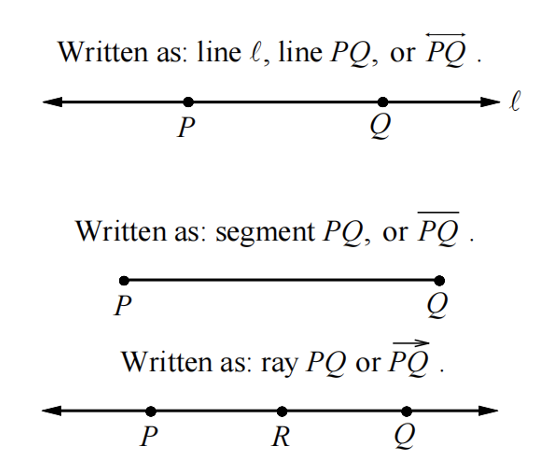
\includegraphics[width=0.55\linewidth]{E8.png}
\end{frame}

\begin{frame}
\section{Angle}
    \begin{tikzpicture}[remember picture, overlay]
        \shade[top color=softPurple, bottom color=softGray] 
            (current page.north west) rectangle (current page.south east);
        \fill[white, opacity=0.3] (current page.center) circle (4cm);
        
        \node[align=center] at (current page.center) {
            {\Huge\bfseries\textcolor{purpleblue}{Angle}} \\[0.5cm]
            {\Large\itshape\textcolor{lightText}{Excellence in SAT Prep}}
        };
        \foreach \x in {1,2,3,4,5} {
            \fill[purpleblue, opacity=0.2] (rand*10-5, rand*7-3.5) circle (0.1+\x*0.05);
        }
        ;
    \end{tikzpicture}
\end{frame}


% Slide 4: Types of Angles
\begin{frame}{Types of Angles}
    \begin{itemize}
        \item \textbf{Acute Angle}: Less than \(90^\circ\).
        \item \textbf{Right Angle}: Exactly \(90^\circ\).
        \item \textbf{Obtuse Angle}: Greater than \(90^\circ\) but less than \(180^\circ\).
        \item \textbf{Straight Angle}: Exactly \(180^\circ\).
        \item \textbf{Reflex Angle}: Greater than \(180^\circ\) but less than \(360^\circ\).
        \item \textbf{Complete Angle}: Exactly \(360^\circ\).
    \end{itemize}

    \centering
    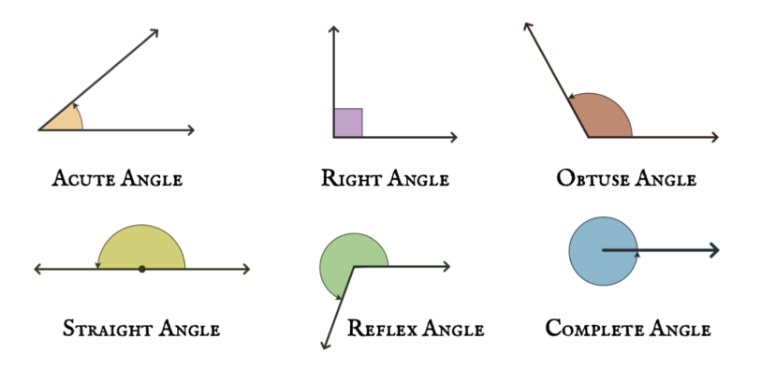
\includegraphics[width=0.8\linewidth]{E9.png}
\end{frame}

% --- Slide: Angle Bisector Theorem ---
\begin{frame}{Angle Bisector Theorem}

    \textbf{Statement:} If a point lies on the \textbf{bisector of an angle}, then it is equidistant from the two sides of the angle.
    
    
    \centering
    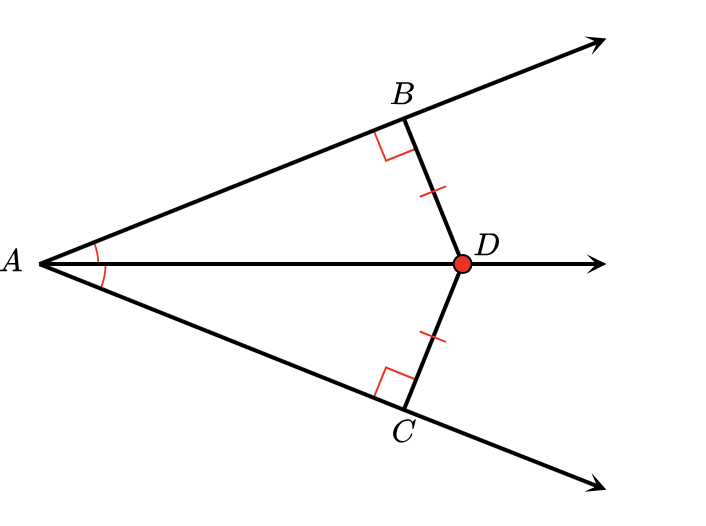
\includegraphics[width=0.35\linewidth]{E11.png}  % Replace with actual image
    
    
    \textbf{Mathematical Representation:}

        \[
        \left\{
        \begin{array}{l}
        \overrightarrow{AD} \text{ bisects } \angle BAC \\
        DB \perp \overrightarrow{AB} \\
        DC \perp \overrightarrow{AC}
        \end{array}
        \right\} \quad \Rightarrow \quad DB = DC
        \]



\end{frame}

\begin{frame}{Exterior Angle Theorem}
\small

\textbf{Theorem Statement:}  
In a triangle, the measure of an \textbf{exterior angle} is equal to the sum of the measures of the two \textbf{remote interior angles}.

\vspace{0.3cm}
\textbf{Visual Representation:}  
If $\angle d$ is the exterior angle , then:
\[
\angle d = \angle a + \angle b
\]

\begin{center}
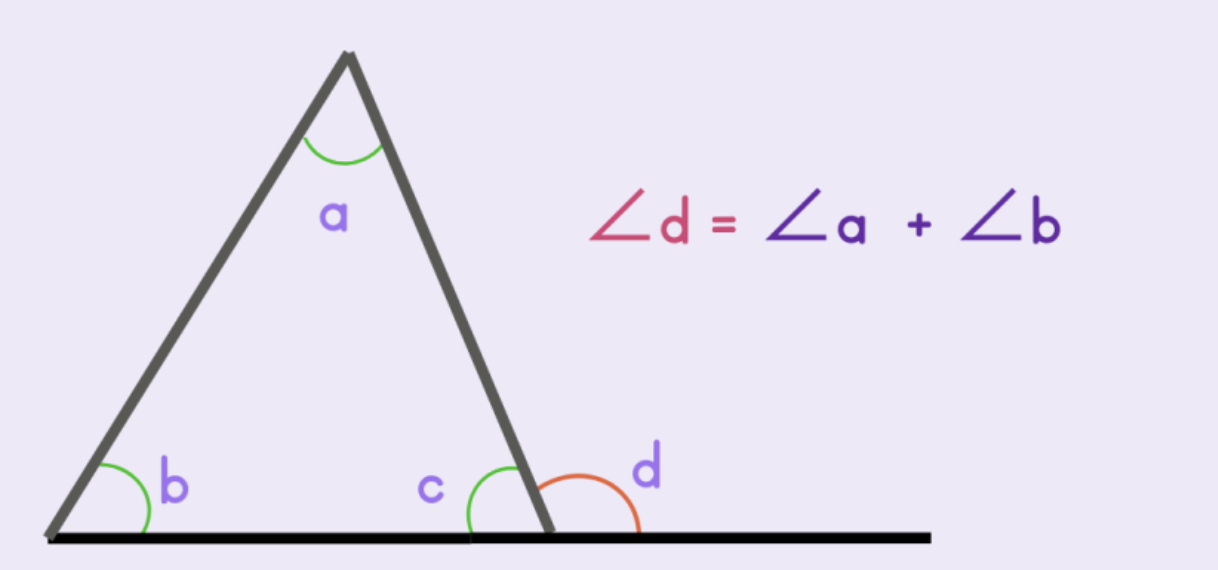
\includegraphics[width=0.6\linewidth]{E41.png} % Replace with actual file if needed
\end{center}



\textbf{SAT Tip:}  
This theorem is frequently used in problems involving triangles and polygon extensions. It’s a shortcut to avoid summing all three triangle angles when only two are needed!

\end{frame}









\begin{frame}{Intersecting Lines and Parallel Lines}
\begin{itemize}


   \item \textbf{Intersecting Lines:} Opposite angles are equal. Also, each pair of angles along the same line adds to \(180^\circ\). In the figure above, \( a + b = 180^\circ \).
    
   \item \textbf{Parallel Lines:} Eight angles are formed when a line crosses two parallel lines. The four large angles (\( a \)) are equal, and the four small angles (\( b \)) are equal.
\end{itemize}

    \begin{center}
        
    
    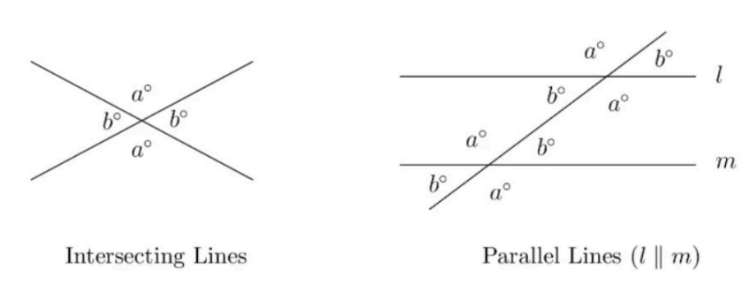
\includegraphics[width=0.85\linewidth]{E10.png}
    \vspace{0.5cm}

    \end{center}
\end{frame}



\begin{frame}{\textbf{Question: Finding Angle Measures}}
    In the figure below, \( \ell \parallel m \), \( r \perp t \), and \( m\angle 1 = 32^\circ \).  
    Lines \( \ell \), \( r \), and \( t \) intersect at one point.  
    \vspace{0.3cm}
    Find \( m\angle 2 \), \( m\angle 3 \), \( m\angle 4 \), and \( m\angle 5 \).

    \begin{center}
        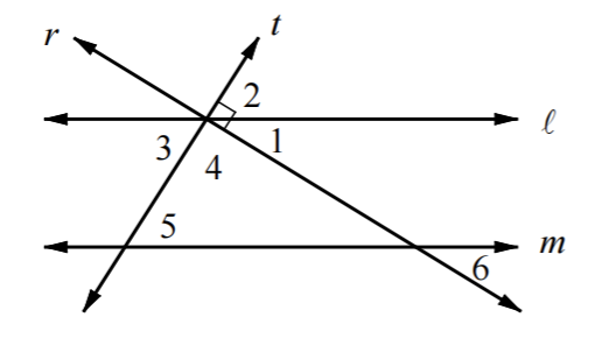
\includegraphics[width=0.6\linewidth]{E12.png} % Replace with the correct file path
    \end{center}
\end{frame}

% --- Answer Explanation ---
\begin{frame}{\textbf{Answer Explanation: Finding Angle Measures}}

    \textbf{Solution:}
    \begin{itemize}
        \item A right angle measures \( 90^\circ \).
        \item Using \( m\angle 1 + m\angle 2 = 90^\circ \):
        \[
        32^\circ + m\angle 2 = 90^\circ
        \]
        \[
        m\angle 2 = 58^\circ
        \]
        \item Vertical angles are congruent:
        \[
        m\angle 2 = m\angle 3 = 58^\circ
        \]
        \item A straight angle measures \( 180^\circ \), so:
        \[
        m\angle 1 + m\angle 4 + m\angle 3 = 180^\circ
        \]
        \[
        32^\circ + m\angle 4 + 58^\circ = 180^\circ
        \]
        \[
        m\angle 4 = 90^\circ
        \]
        \item Alternate interior angles are congruent:
        \[
        m\angle 3 = m\angle 5 = 58^\circ
        \]
    \end{itemize}

\end{frame}

\begin{frame}{\textbf{Answer Explanation: Finding Angle Measures}}

    \begin{itemize}
        \item Corresponding angles are congruent:
        \[
        m\angle 1 = m\angle 6 = 32^\circ
        \]

    \textbf{Final Answers:}  
    \[
    m\angle 2 = 58^\circ, \quad m\angle 3 = 58^\circ, \quad m\angle 4 = 90^\circ, \quad m\angle 5 = 58^\circ.
    \]
    \end{itemize}
    
\end{frame}


\begin{frame}{\textbf{Question: Finding \( \angle TUR \)}}
    In the figure shown, points \( Q, R, S, \) and \( T \) lie on line segment \( PV \),  
    and line segment \( RU \) intersects line segment \( SX \) at point \( W \).

    \vspace{0.3cm}
    Given:
    \begin{itemize}
        \item \( \angle SQX = 48^\circ \)
        \item \( \angle SXQ = 86^\circ \)
        \item \( \angle SWU = 85^\circ \)
        \item \( \angle VTU = 162^\circ \)
    \end{itemize}

    What is the measure, in degrees, of \( \angle TUR \)?

    \begin{center}
        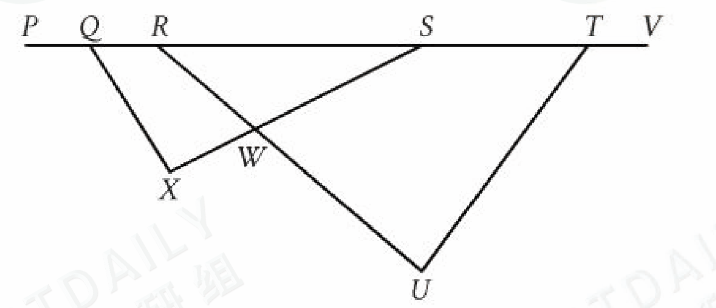
\includegraphics[width=0.6\linewidth]{E13.png} % Replace with the correct file path
    \end{center}

\end{frame}



% --- Answer Explanation ---
\begin{frame}{\textbf{Answer Explanation: Finding \( \angle TUR \)}}
    \textbf{Solution:}
    \begin{itemize}
        \item Compute \( \angle XQS \) using the given angles:
        \[
        \angle XQS = 180^\circ - \angle SXQ = 180^\circ - 86^\circ = 94^\circ
        \]
        \item Compute \( \angle XSW \) using \( \angle SQX \) and \( \angle XQS \):
        \[
        \angle XSW = 180^\circ - (\angle SQX + \angle XQS) = 180^\circ - (48^\circ + 94^\circ) = 38^\circ
        \]
        \item Use \( \angle SWU = 85^\circ \) to find \( \angle WUR \):
        \[
        \angle WUR = 180^\circ - (\angle SWU + \angle XSW) = 180^\circ - (85^\circ + 38^\circ) = 57^\circ
        \]
        \item Compute \( \angle TUR \) using \( \angle VTU = 162^\circ \):
        \[
        \angle TUR = 180^\circ - \angle WUR = 180^\circ - 57^\circ = 123^\circ
        \]
    \end{itemize}

    \textbf{Final Answer:} \( \boxed{123^\circ} \).

\end{frame}


\begin{frame}{Polygons and Interior Angles}
\small
\begin{center}
    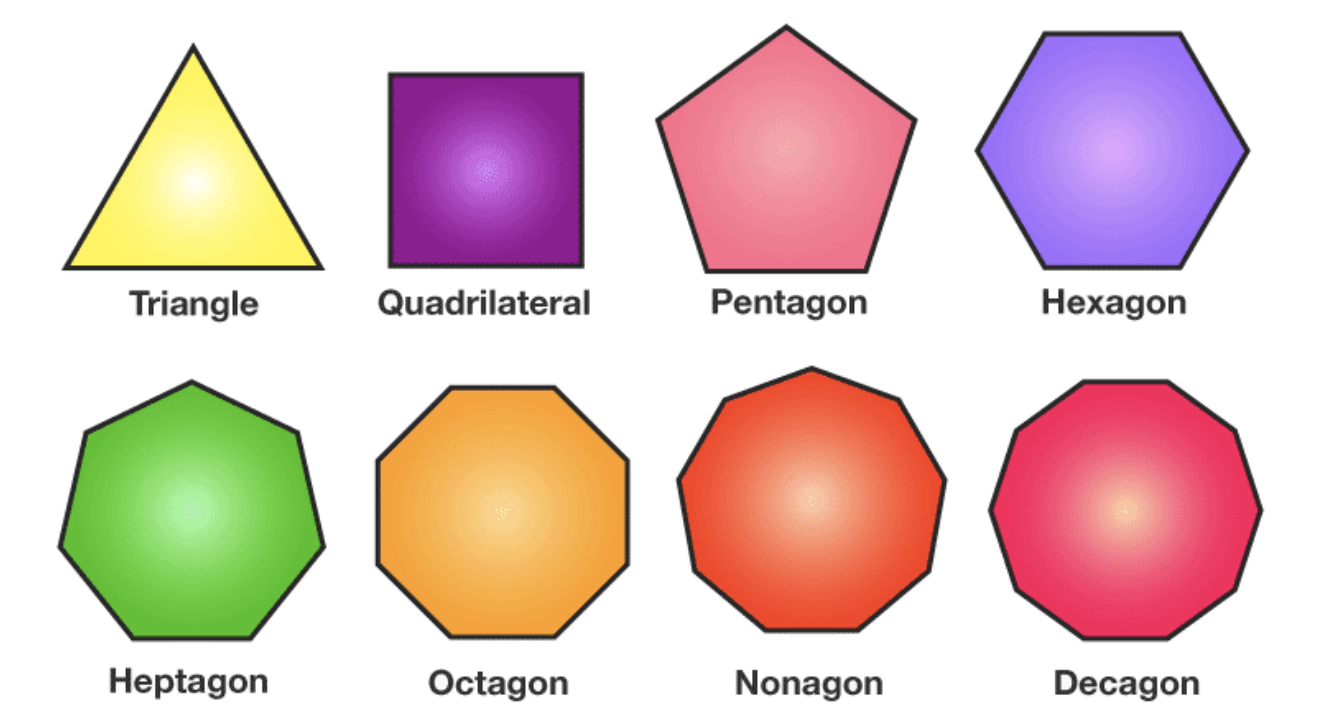
\includegraphics[width = 0.3\linewidth]{E40.png}
\end{center}

\textbf{Polygon Angle Sum Formula:}
\[
\text{Sum of interior angles} = 180^\circ(n - 2)
\]
\begin{itemize}
    \item $n$ = number of sides
    \item Each additional side increases the angle sum by $180^\circ$
\end{itemize}

\vspace{0.2cm}
\textbf{Regular Polygon:}  


All sides and angles are equal.

\textbf{Measure of Each Interior Angle in a Regular Polygon:}
\[
\text{Each angle} = \frac{180(n - 2)}{n}
\]



\end{frame}

\begin{frame}{\textbf{Question: Polygon Angle Problem}}
\small

A regular polygon has an interior angle that is 4 times the exterior plus 60 the measure of its exterior angle. 

\vspace{0.3cm}
\textbf{Question:}  
How many sides does the polygon have?

\vspace{0.4cm}
\textbf{Choices:}
\begin{itemize}
    \item[A.] 9
    \item[B.] 10
    \item[C.] 12
    \item[D.] 15
\end{itemize}

\end{frame}
\begin{frame}{\textbf{Answer and Explanation}}



"A regular polygon has an interior angle that is 60 more than four times its exterior angle."

Then:
\[
x = 4y + 60,\quad x + y = 180
\Rightarrow 4y + 60 + y = 180

\]

✅ \textbf{Correct Answer: D. 15}

\end{frame}



\begin{frame}
\section{Triangle}
    \begin{tikzpicture}[remember picture, overlay]
        \shade[top color=softPurple, bottom color=softGray] 
            (current page.north west) rectangle (current page.south east);
        \fill[white, opacity=0.3] (current page.center) circle (4cm);
        
        \node[align=center] at (current page.center) {
            {\Huge\bfseries\textcolor{purpleblue}{Triangle}} \\[0.5cm]
            {\Large\itshape\textcolor{lightText}{Excellence in SAT Prep}}
        };
        \foreach \x in {1,2,3,4,5} {
            \fill[purpleblue, opacity=0.2] (rand*10-5, rand*7-3.5) circle (0.1+\x*0.05);
        }
        ;
    \end{tikzpicture}
\end{frame}


\begin{frame}{Isosceles and Equilateral Triangles}
\small

\textbf{Isosceles Triangle:}
\begin{itemize}
    \item Has two equal sides.
    \item The angles opposite the equal sides are also equal.
    \item Often appears in SAT triangle congruence or symmetry problems.
\end{itemize}

\vspace{0.3cm}
\textbf{Equilateral Triangle:}
\begin{itemize}
    \item All sides are equal.
    \item Each angle measures $60^\circ$.
    \item Always a regular polygon.
\end{itemize}

\begin{center}
    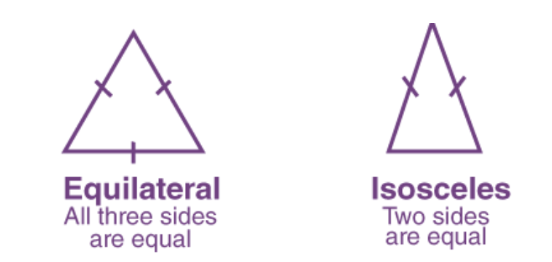
\includegraphics[width=0.5\linewidth]{E42.png}
\end{center}

\end{frame}


\begin{frame}{\textbf{Question: Area of Equilateral Triangles }}
\begin{center}
    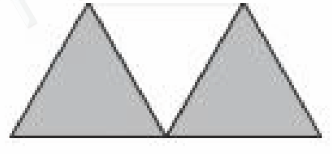
\includegraphics[width=0.3\linewidth]{E47.png}
\end{center}

A graphic designer is creating a logo for a company. The logo is shown in the figure above. The logo is in the shape of a trapezoid and consists of three congruent equilateral triangles. 

If the perimeter of the logo is 20 centimeters, what is the combined area of the shaded regions, in square centimeters, of the logo?

\begin{itemize}
    \item[A.] \( 2\sqrt{3} \)
    \item[B.] \( 4\sqrt{3} \)
    \item[C.] \( 8\sqrt{3} \)
    \item[D.] \( 16 \)
\end{itemize}
\end{frame}


\begin{frame}{\textbf{Answer: Area of Equilateral Triangles in a Logo}}



In the diagram, the trapezoid has **4 edges**, and each triangle has 3 sides. The full figure has:
\[
\text{Perimeter} = 5s \Rightarrow 5s = 20 \Rightarrow s = 4
\]

Area of one triangle:
\[
A = \frac{\sqrt{3}}{4}(4)^2 = \frac{\sqrt{3}}{4}(16) = 4\sqrt{3}
\]

Two shaded triangles:
\[
2 \cdot 4\sqrt{3} = 8\sqrt{3}
\]

\textbf{Correct Answer:} \fbox{\( \text{C. } 8\sqrt{3} \)}
\end{frame}


\begin{frame}{Circumcenter of a Triangle}

\textbf{Key Concepts:}
\begin{itemize}
    \item The \textbf{circumcenter} (denoted as $T$) is the point where the \textbf{perpendicular bisectors} of a triangle intersect.
    \item The circumcenter is \textbf{equidistant} from all three vertices of the triangle:
    \[
    TQ = TP = TR
    \]
    \item This implies that in any triangle $\triangle PQR$:
    \[
    TQ = TP = TR = \text{circumradius}
    \]
    \item In coordinate geometry, the circumcenter can be found as the intersection point of the perpendicular bisectors of any two sides.
\end{itemize}


\begin{center}
    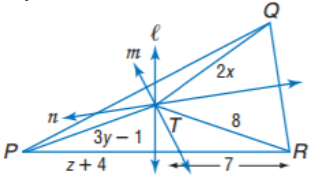
\includegraphics[width=0.3\linewidth]{E78.png}
\end{center}


\end{frame}



\begin{frame}{Medial Triangle Theorem}

\textbf{Key Concepts:}
\begin{itemize}
    \item The \textbf{midpoints of a triangle} are the points where each side is bisected, meaning each side is divided into two equal segments.
    \item Connecting the midpoints of a triangle forms a \textbf{medial triangle}.
    \item The medial triangle is:
    \begin{itemize}
        \item Parallel to the original triangle.
        \item Has sides that are half the length of the corresponding sides of the original triangle.
    \end{itemize}
    \item This theorem is useful in geometry proofs and helps simplify complex triangle problems.
\end{itemize}

\begin{center}
    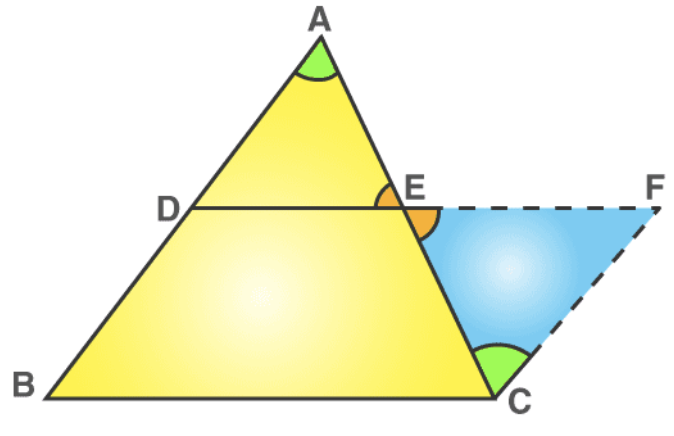
\includegraphics[width=0.3\linewidth]{E79.png}
\end{center}

\end{frame}




\begin{frame}{Right Triangles}
\small
\begin{columns}
    \begin{column}{0.45\textwidth}

\textbf{Definition:} A triangle with one $90^\circ$ angle.

\vspace{0.3cm}
\textbf{Pythagorean Theorem:}
\[
a^2 + b^2 = c^2
\]
Where $a$ and $b$ are legs and $c$ is the hypotenuse.

\vspace{0.3cm}
\textbf{Pythagorean Triples (SAT favorites):}
\begin{itemize}
    \item $(3, 4, 5)$
    \item $(5, 12, 13)$
\end{itemize}
\end{column}

    \begin{column}{0.56\textwidth}
        \centering
        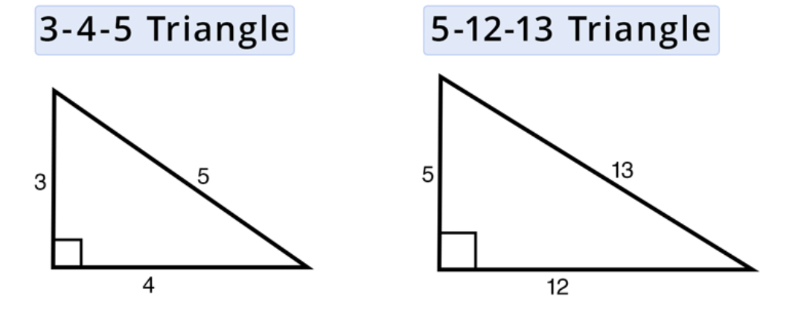
\includegraphics[width=\linewidth]{E44.png} % replace with your actual file name
    \end{column}
\end{columns}
\end{frame}

\begin{frame}{Special Right Triangles}
\small
\begin{columns}
    \begin{column}{0.45\textwidth}
        \textbf{1. 45°-45°-90° Triangle}
        \begin{itemize}
            \item Legs are equal.
            \item Hypotenuse: $x\sqrt{2}$ if each leg is $x$.
        \end{itemize}

        \vspace{0.3cm}
        \textbf{2. 30°-60°-90° Triangle}
        \begin{itemize}
            \item Short leg: $x$
            \item Long leg: $x\sqrt{3}$
            \item Hypotenuse: $2x$
        \end{itemize}
    \end{column}
    
    \begin{column}{0.56\textwidth}
        \centering
        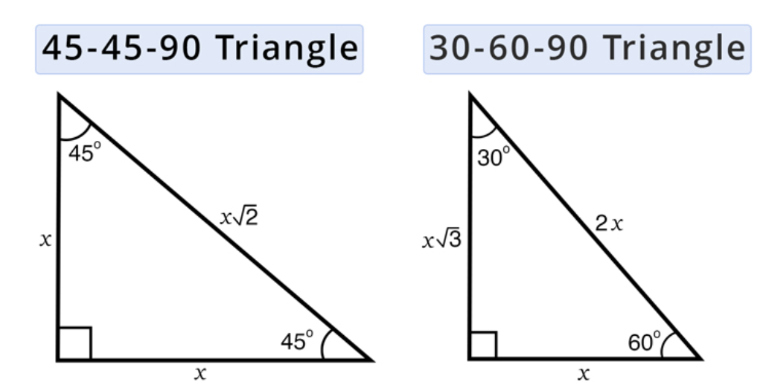
\includegraphics[width=\linewidth]{E43.png} % replace with your actual file name
    \end{column}
\end{columns}
\end{frame}

\begin{frame}{\textbf{Question: Geometry – Right Triangle with Altitude}}
In triangle \( \triangle ABC \), the measure of angle \( B \) is \( 90^\circ \), and \( \overline{BD} \) is an altitude of the triangle.

\begin{itemize}
    \item The length of \( \overline{AB} \) is \( 15 \),
    \item The length of \( \overline{AC} \) is \( 23 \) greater than the length of \( \overline{AB} \),
\end{itemize}

What is the value of \( \dfrac{BC}{BD} \)?

\begin{itemize}
    \item[A.] \( \dfrac{15}{38} \)
    \item[B.] \( \dfrac{15}{23} \)
    \item[C.] \( \dfrac{23}{15} \)
    \item[D.] \( \dfrac{38}{15} \)
\end{itemize}
\end{frame}
\begin{frame}{\textbf{Answer: Geometry – Right Triangle }}

We are given:
\begin{itemize}
    \item \( AB = 15 \)
    \item \( AC = AB + 23 = 15 + 23 = 38 \)
    \item \( \angle B = 90^\circ \), so triangle \( \triangle ABC \) is a right triangle.
\end{itemize}

Using the Pythagorean Theorem:
\[
AB^2 + BC^2 = AC^2 \Rightarrow 15^2 + BC^2 = 38^2
\]


\textbf{Correct Answer:} \fbox{D. \( \dfrac{38}{15} \)}
\end{frame}


\begin{frame}{Congruent Triangles: Definition and Proof }
\small

\textbf{Definition:}  
Two triangles are \textbf{congruent} if all corresponding sides and angles are equal. That means:
\[
\text{Side} = \text{Side},\quad \text{Angle} = \text{Angle}
\]
\[
\triangle ABC \cong \triangle DEF \quad \Rightarrow \quad AB = DE,\ \angle A = \angle D,\ \text{etc.}
\]

\vspace{0.3cm}
\textbf{Methods to Prove Triangle Congruence:}
\begin{itemize}
    \item \textbf{SSS (Side-Side-Side):} All three sides of one triangle are equal to the corresponding sides of another.
    \item \textbf{SAS (Side-Angle-Side):} Two sides and the included angle are congruent.
    \item \textbf{ASA (Angle-Side-Angle):} Two angles and the included side are congruent.

    \item \textbf{HL (Hypotenuse-Leg):} In right triangles, hypotenuse and one leg are congruent.
\end{itemize}

\vspace{0.2cm}
\textbf{SAT Tip:}  
Do \textbf{not} assume triangle congruence from AAA or SSA — these are not valid for proving congruence.

\end{frame}



\begin{frame}{\textbf{Question: Triangle Congruence}}
In triangles \( ABC \) and \( DEF \), angles \( B \) and \( E \) each have measure \( 27^\circ \), and angles \( C \) and \( F \) each have measure \( 41^\circ \). 

Which additional piece of information is sufficient to determine whether triangle \( ABC \) is congruent to triangle \( DEF \)?

\begin{itemize}
    \item[A.] The measure of angle \( A \)
    \item[B.] The length of side \( AB \)
    \item[C.] The lengths of sides \( BC \) and \( EF \)
    \item[D.] No additional information is necessary
\end{itemize}
\end{frame}


\begin{frame}{\textbf{Answer: Triangle Congruence}}
Since two angles are known in each triangle:
\[
\angle B = \angle E = 27^\circ, \quad \angle C = \angle F = 41^\circ
\]
We can determine the third angle because the angles of a triangle sum to \(180^\circ\):
\[
\angle A = \angle D = 180^\circ - 27^\circ - 41^\circ = 112^\circ
\]

Therefore, all three angles in both triangles are known and equal:
\[
\angle A = \angle D, \quad \angle B = \angle E, \quad \angle C = \angle F
\]

Thus, the two triangles are similar (AAA), but to determine \textbf{congruence}, one side must be known.

If one side length (e.g., \( AB \)) is known, the Side-Angle-Angle (ASA) or Angle-Side-Angle (ASA) congruence criterion can be applied.

\textbf{Answer:} \fbox{C}
\end{frame}





\begin{frame}{Similar Triangles}
\small
\begin{columns}
    \begin{column}{0.45\textwidth}

\textbf{Definition:}
Triangles are similar if their corresponding angles are equal and corresponding sides are in proportion.

\vspace{0.3cm}
\textbf{Symbolically:} $\triangle BAC \sim \triangle BDE$

\vspace{0.3cm}
\textbf{Properties:}
\begin{itemize}
    \item All corresponding angles are equal.
    \item All corresponding sides are proportional.
    \item $\frac{DB}{AB} = \frac{BE}{BC} = \frac{DE}{AC}$
\end{itemize}

\vspace{0.3cm}
\textbf{SAT Tip:}
Use proportions to solve for missing side lengths or establish ratios between parts of a figure.


\end{column}

    \begin{column}{0.4\textwidth}
        \centering
        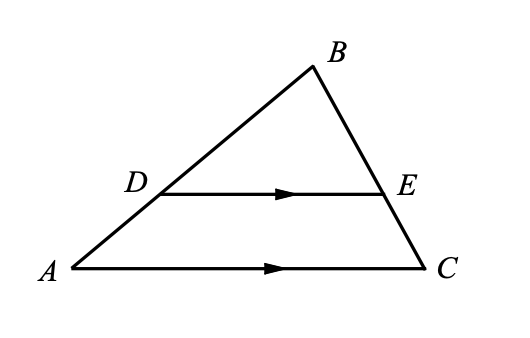
\includegraphics[width=\linewidth]{E45.png} % replace with your actual file name
    \end{column}
\end{columns}
\end{frame}


\begin{frame}{Similar Triangles: Definition and Proof Methods}
\small

\textbf{Definition:}  
Two triangles are \textbf{similar} if their corresponding angles are equal and their corresponding sides are in proportion.

\[
\triangle ABC \sim \triangle DEF \quad \Rightarrow \quad \angle A = \angle D,\ \angle B = \angle E,\ \angle C = \angle F
\]
\[
\frac{AB}{DE} = \frac{BC}{EF} = \frac{AC}{DF}
\]

\vspace{0.3cm}
\textbf{Ways to Prove Similar Triangles:}
\begin{itemize}
    \item \textbf{AA (Angle-Angle):} If two angles of one triangle are equal to two angles of another, the triangles are similar.
    \item \textbf{SSS (Side-Side-Side) Similarity:} If all three pairs of corresponding sides are in proportion.
    \item \textbf{SAS (Side-Angle-Side) Similarity:} If two sides are in proportion and the included angle is equal.
\end{itemize}
\end{frame}


\begin{frame}{\textbf{Question: Triangle Similarity Criterion}}
In triangles \( LMN \) and \( RST \), angles \( L \) and \( R \) each have measure \( 60^\circ \), \( LN = 10 \), and \( RT = 30 \). 

Which additional piece of information is sufficient to prove that triangle \( LMN \) is similar to triangle \( RST \)?

\begin{itemize}
    \item[A.] \( MN = 7 \) and \( ST = 7 \)
    \item[B.] \( MN = 7 \) and \( ST = 21 \)
    \item[C.] The measures of angles \( M \) and \( S \) are \( 70^\circ \) and \( 60^\circ \), respectively
    \item[D.] The measures of angles \( M \) and \( T \) are \( 70^\circ \) and \( 50^\circ \), respectively
\end{itemize}
\end{frame}


\begin{frame}{\textbf{Answer: Triangle Similarity Criterion}}


\textbf{Answer:} \fbox{D}
\end{frame}




\begin{frame}{Similar Triangles in Right Triangle Model}
\small
\begin{columns}
    \begin{column}{0.6\textwidth}
        \textbf{Concept:}  
        In a right triangle, when an altitude is drawn from the right angle to the hypotenuse, it creates two smaller triangles that are similar to the original triangle and to each other.

        \vspace{0.2cm}
        \textbf{Proportional Relationship:}
        \[
        \frac{a}{h} = \frac{h}{b}
        \quad \Rightarrow \quad
        h = \sqrt{ab}
        \]
        where:
        \begin{itemize}
            \item $a$ and $b$ are the segments of the hypotenuse,
            \item $h$ is the altitude to the hypotenuse.
        \end{itemize}

        \vspace{0.2cm}

        \textbf{Tip:}  
        This model leads to fast solutions when given two sides and asked for height or area.
    \end{column}

    \begin{column}{0.38\textwidth}
        \centering
        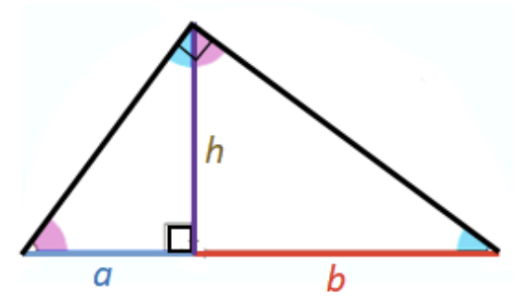
\includegraphics[width=\linewidth]{E46.png}
    \end{column}
\end{columns}
\end{frame}


\begin{frame}{\textbf{Question: Triangle Area and Geometry Constraints}}
\begin{center}
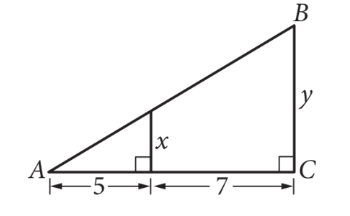
\includegraphics[width=0.4\textwidth]{E49.png}
\end{center}



Given:
\begin{itemize}
    \item The area of triangle \( ABC \) is at least 48 but no more than 60.
    \item \( y \) is an integer.
\end{itemize}

What is one possible value of \( x \)?
\end{frame}

\begin{frame}{\textbf{Answer: Triangle Area and Geometry Constraints}}
We are given:
\[
\text{Area} = \frac{1}{2} \times \text{base} \times \text{height}
= \frac{1}{2} \times 12 \times y = 6y
\]
\[
48 \leq 6y \leq 60
\Rightarrow 8 \leq y \leq 10
\]
So possible integer values for \( y \) are \( 8, 9, \) or \( 10 \).

We are told that \( x \) is the distance from point \( A \) to where the perpendicular from \( B \) hits base \( AC \), which lies between \( A \) and \( C \). Since \( AC = 12 \), one possible value of \( x \) that lies between 0 and 12 is:
\[
\boxed{\frac{25}{6}}
\]

\textbf{Possible Answer:} \fbox{5}
\end{frame}




\begin{frame}{\textbf{Question: Right Triangle Segment Length}}
\begin{center}
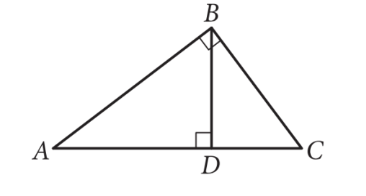
\includegraphics[width=0.35\textwidth]{E50.png}
\end{center}

In the figure above:
\begin{itemize}
    \item \( BD = 6 \)
    \item \( AD = 8 \)
\end{itemize}

What is the length of \( \overline{DC} \)?
\end{frame}

\begin{frame}{\textbf{Answer: Right Triangle Segment Length}}


\textbf{Answer:} \fbox{4.5}
\end{frame}




\begin{frame}{\textbf{Question: Right Triangle Geometry}}
\begin{center}
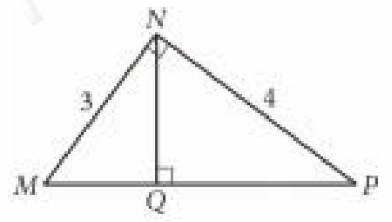
\includegraphics[width=0.40\linewidth]{E48.png}
\end{center}

In the figure above, what is the length of segment \( \overline{NQ} \)?

\begin{itemize}
    \item[A.] \( 2.2 \)
    \item[B.] \( 2.3 \)
    \item[C.] \( 2.4 \)
    \item[D.] \( 2.5 \)
\end{itemize}
\end{frame}
\begin{frame}{\textbf{Answer: Right Triangle Geometry}}


Use the full triangle \( \triangle MNP \) with legs \( MN = 3 \) and \( NP = 4 \). That makes \( MP \) the hypotenuse:
\[
MP^2 = MN^2 + NP^2 = 3^2 + 4^2 = 9 + 16 = 25 \Rightarrow MP = 5
\]

So triangle \( \triangle MNP \) is a right triangle with hypotenuse 5. Since \( \angle MQN \) is a right angle, \( NQ \) is the height to the hypotenuse.

Area of triangle using base and height:
\[
\text{Area} = \frac{1}{2} \cdot MP \cdot NQ = \frac{1}{2} \cdot 5 \cdot NQ
\]

Area using two legs:
\[
\text{Area} = \frac{1}{2} \cdot 3 \cdot 4 = 6
\]

Equating both:
\[
\frac{1}{2} \cdot 5 \cdot NQ = 6 \Rightarrow \frac{5}{2} \cdot NQ = 6 \Rightarrow NQ = \frac{12}{5} = 2.4
\]

\textbf{Correct Answer:} \fbox{C. \( 2.4 \)}
\end{frame}


\begin{frame}

\section{Cube, Rectangle, rhombus, parallelogram}
    \begin{tikzpicture}[remember picture, overlay]
        \shade[top color=softPurple, bottom color=softGray] 
            (current page.north west) rectangle (current page.south east);
        \fill[white, opacity=0.3] (current page.center) circle (4cm);
        
        \node[align=center] at (current page.center) {
            {\Large\bfseries\textcolor{purpleblue}{Cube, Rectangle, rhombus, parallelogram}} \\[0.5cm]
            {\Large\itshape\textcolor{lightText}{Excellence in SAT Prep}}
        };
        \foreach \x in {1,2,3,4,5} {
            \fill[purpleblue, opacity=0.2] (rand*10-5, rand*7-3.5) circle (0.1+\x*0.05);
        }
        ;
    \end{tikzpicture}
\end{frame}

\begin{frame}{Parallelogram: Properties and Proof}
\textbf{Properties:}
\begin{itemize}
    \item Opposite sides are parallel: $AB \parallel CD$, $AD \parallel BC$.
    \item Opposite sides are congruent: $AB = CD$, $AD = BC$.
    \item Opposite angles are congruent: $\angle A = \angle C$, $\angle B = \angle D$.
    \item Diagonals bisect each other: $AO = OC$, $BO = OD$ (where $O$ is the intersection point).
\end{itemize}

\vspace{1em}
\textbf{Proof Ideas:}
\begin{itemize}
    \item Use triangle congruence (e.g., ASA, SAS) to prove sides and angles.
    \item Use parallel line theorems (alternate interior angles).
    \item Show that diagonals bisect each other using congruent triangles.
\end{itemize}
\end{frame}

% Frame 2 - Rhombus
\begin{frame}{Rhombus: Properties and Proof}
\textbf{Properties:}
\begin{itemize}
    \item All sides are congruent: $AB = BC = CD = DA$.
    \item Opposite sides are parallel.
    \item Diagonals bisect each other at right angles: $AC \perp BD$.
    \item Diagonals bisect opposite angles.
\end{itemize}

\vspace{1em}
\textbf{Proof Ideas:}
\begin{itemize}
    \item Use parallelogram properties plus congruent sides.
    \item Prove diagonals are perpendicular using congruent triangles (e.g., SSS).
    \item Show angle bisection using diagonal properties and symmetry.
\end{itemize}
\end{frame}

% Frame 3 - Square
\begin{frame}{Square: Properties and Proof}
\textbf{Properties:}
\begin{itemize}
    \item All sides are congruent: $AB = BC = CD = DA$.
    \item All angles are right angles: $\angle A = \angle B = \angle C = \angle D = 90^\circ$.
    \item Diagonals are congruent and perpendicular.
    \item Diagonals bisect opposite angles.
\end{itemize}

\vspace{1em}
\textbf{Proof Ideas:}
\begin{itemize}
    \item Use properties of both a rectangle and a rhombus.
    \item Show all sides are equal using SSS or coordinate geometry.
    \item Show diagonals are perpendicular and congruent using triangle congruence.
\end{itemize}
\end{frame}

% Frame 4 - Rectangle
\begin{frame}{Rectangle: Properties and Proof}
\textbf{Properties:}
\begin{itemize}
    \item Opposite sides are congruent and parallel.
    \item All angles are right angles.
    \item Diagonals are congruent and bisect each other.
\end{itemize}

\vspace{1em}
\textbf{Proof Ideas:}
\begin{itemize}
    \item Use parallelogram properties plus right angles.
    \item Show all angles are right using parallel lines and transversal properties.
    \item Use congruent triangles to prove diagonals are equal.
\end{itemize}
\end{frame}


\begin{frame}
\section{Practices}
    \begin{tikzpicture}[remember picture, overlay]
        \shade[top color=softPurple, bottom color=softGray] 
            (current page.north west) rectangle (current page.south east);
        \fill[white, opacity=0.3] (current page.center) circle (4cm);
        
        \node[align=center] at (current page.center) {
            {\Huge\bfseries\textcolor{purpleblue}{Practices}} \\[0.5cm]
            {\Large\itshape\textcolor{lightText}{Excellence in SAT Prep}}
        };
        \foreach \x in {1,2,3,4,5} {
            \fill[purpleblue, opacity=0.2] (rand*10-5, rand*7-3.5) circle (0.1+\x*0.05);
        }
        ;
    \end{tikzpicture}
\end{frame}





\begin{frame}{Transversal Angles and Parallel Lines}
\textbf{Question:}
In the figure below, lines \( l \) and \( m \) are parallel.

\begin{center}
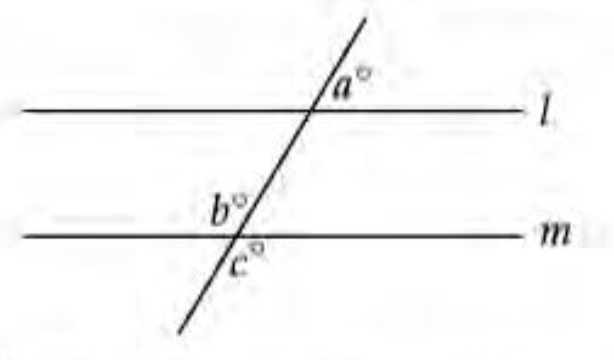
\includegraphics[width=0.4\textwidth]{E77.png}
\end{center}

If \( b = 9k + 15 \) and \( c = 16k - 76 \), what is the value of \( a \)?
\end{frame}


\begin{frame}{Solution}
\textbf{Solution:}


\textbf{Answer:} \( a = 48^\circ \).
\end{frame}

\begin{frame}{Area of an Isosceles Right Triangle}
\textbf{Question:}
The hypotenuse of an isosceles right triangle has a length of \( 12 \) units. What is the area of the triangle, in square units?

\begin{itemize}
    \item[A]\( 18\sqrt{2} \)
    \item[B]\( 36 \)
    \item[C]\( 48 \)
    \item[D] \( 36\sqrt{2} \)
    


\end{itemize}
\end{frame}

\begin{frame}{Solution}
\textbf{Solution:}
\begin{itemize}
    \item Let the length of each leg of the isosceles right triangle be \( x \).
    \item Then:
    \[
    x^2 + x^2 = 12^2
    \]
    \[
    2x^2 = 144
    \]
    \[
    x^2 = 72
    \]
    \[
    x = 6\sqrt{2}
    \]
    \item Therefore, the area is:
    \[
    A = \frac{1}{2} \times x \times x = \frac{1}{2} \times (6\sqrt{2}) \times (6\sqrt{2}) = \frac{1}{2} \times 72 = 36
    \]
\end{itemize}
\textbf{Answer:} \( \boxed{36} \)
\end{frame}


\begin{frame}{Similarity of Triangles}
\textbf{Question:}
In triangles \(LMN\) and \(RST\), angles \(L\) and \(R\) each have measure \(127^\circ\). Which additional piece of information is sufficient to determine whether triangle \(LMN\) is similar to triangle \(RST\)?
\begin{choices}
\choice The measures of angles \(N\) and \(T\).
\choice The lengths of sides \(LM\) and \(RS\).
\choice The measures of angles \(S\) and \(T\).
\choice The lengths of sides \(MN\) and \(ST\).
\end{choices}
\end{frame}


\begin{frame}{Solution}
\textbf{Solution:}
To determine whether two triangles are similar, we need:
\begin{itemize}
    \item Two pairs of corresponding angles to be congruent (AA~criterion).
    \item Alternatively, corresponding sides to be proportional (SSS~or~SAS~criterion).
\end{itemize}
Given \( \angle L = \angle R = 127^\circ \):
\begin{itemize}
    \item Knowing either \( \angle N \) and \( \angle T \) or \( \angle S \) and \( \angle T \) would be sufficient by AA criterion.
\end{itemize}
Therefore:
\[
\boxed{\text{Option A: The measures of angles } N \text{ and } T}
\]
\end{frame}


\begin{frame}{Similarity of Triangles}
\textbf{Question:}
In triangles \(LMN\) and \(RST\), angles \(L\) and \(R\) each have measure \(127^\circ\). Which additional piece of information is sufficient to determine whether triangle \(LMN\) is similar to triangle \(RST\)?
\begin{itemize}
    \item[A]The measures of angles \(N\) and \(T\).
    \item[B] The lengths of sides \(LM\) and \(RS\).
    \item[C]The measures of angles \(S\) and \(T\).
    \item[D]The lengths of sides \(MN\) and \(ST\).


\end{itemize}
\end{frame}


\begin{frame}{Solution}
\textbf{Solution:}
To determine whether two triangles are similar, we need:
\begin{itemize}
    \item Two pairs of corresponding angles to be congruent (AA~criterion).
    \item Alternatively, corresponding sides to be proportional (SSS~or~SAS~criterion).
\end{itemize}
Given \( \angle L = \angle R = 127^\circ \):
\begin{itemize}
    \item Knowing either \( \angle N \) and \( \angle T \) or \( \angle S \) and \( \angle T \) would be sufficient by AA criterion.
\end{itemize}
Therefore:
\[
\boxed{\text{Option A: The measures of angles } N \text{ and } T}
\]
\end{frame}


\begin{frame}{Congruence of Triangles}
\textbf{Question:}
In triangles \(LMN\) and \(PQR\), angles \(M\) and \(Q\) each have measure \(54^\circ\), \(MN = 16\), and \(QR = 16\). Which additional piece of information is sufficient to prove that triangle \(LMN\) is congruent to triangle \(PQR\)?

\vspace{1em}
\textbf{Answer Choices:}
\begin{itemize}
    \item[A] Angles \(L\) and \(R\) each have measure \(44^\circ\).
    \item[B] Angles \(N\) and \(P\) each have measure \(44^\circ\).
    \item[C] \(LM = 11\) and \(PQ = 11\).
    \item[D] \(LN = 11\) and \(PR = 11\).
\end{itemize}
\end{frame}

\begin{frame}{Question}

C
    
\end{frame}










\begin{frame}{}
    \begin{tikzpicture}[remember picture, overlay]
        % 背景渐变色：蓝紫到白
        \shade[top color=novelPurple!40, bottom color=white]
            (current page.north west) rectangle (current page.south east);

        % 中心柔光
        \fill[white, opacity=0.15] (current page.center) circle (5cm);

        % 柔和光点点缀
        \foreach \x in {1,2,3,4,5} {
            \fill[novelPurple, opacity=0.12] (rand*10-5, rand*7-3.5) circle (0.1+\x*0.05);
        }
    \end{tikzpicture}

    \centering
    \vspace{5em}

    {\Huge \textbf{\textcolor{novelPurple}{Thank You!}}} \\[1em]
    {\large \textcolor{gray}{We appreciate your time and focus.}} \\[3em]

    {\LARGE \textbf{\textcolor{novelPurple}{\textsf{Novel Prep}}}}

    \vfill
\end{frame}























\end{document}